Consider the following feedback system.	
\begin{center}
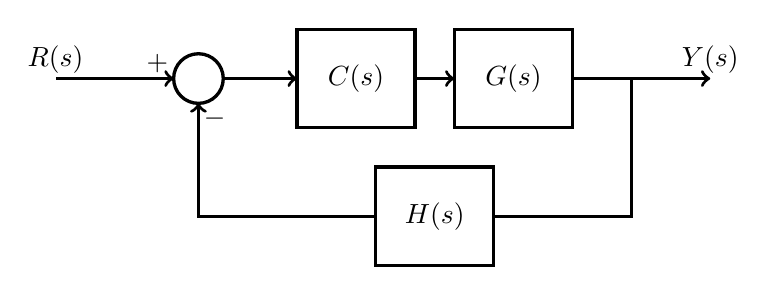
\begin{tikzpicture}[scale=1,inner sep=0pt,outer sep=0pt,very thick,
sysblock/.style={draw,rectangle,inner sep=2pt,minimum width=1.5cm,minimum height=1.25cm,very thick}]
\draw (3,0) node[draw,circle] (sum3) {$\rule{0pt}{18pt}$};
%\draw (7,0) node[draw,circle] (sum2) {$\rule{0pt}{18pt}$};
\draw (5,0) node[sysblock] (C) {$C(s)$};
\draw (7,0) node[sysblock] (G) {$G(s)$};
\draw (6,-1.75) node[sysblock] (Kd) {$H(s)$};

\draw[<-] (sum3.180)  node[above left=2pt] {$+$} -- ++(-1.5,0) node[above=2pt] {$R(s)$};
\draw[->] (sum3.0) -- (C);
\draw[->] (C) -- (G);
\draw[->] (G) -- ++(2.5,0) node[above=2pt] {$Y(s)$};
\draw[->] (G) ++(1.5,0) |- (Kd) -| (sum3.-90) node[below right=2pt] {$-$};
%\draw[<-] (sum2.90) node[above right=2pt] {$+$} -- ++(0,1) node[right=2pt] {$D(s)$};
\end{tikzpicture}
\end{center}
By hand, sketch the Bode plots and Nyquist plots for the loop gain $L(s) = H(s)G(s)C(s) = \frac{(s-5)}{(s+10)}$. Determine if the closed loop system is stable.

